\appendix
%% Правка оформления ссылок на приложения:
%http://tex.stackexchange.com/questions/56839/chaptername-is-used-even-for-appendix-chapters-in-toc
%http://tex.stackexchange.com/questions/59349/table-of-contents-with-chapter-and-appendix
%% требует двойной компиляции
\addtocontents{toc}{\def\protect\cftchappresnum{\appendixname{} }%
\setlength{\cftchapnumwidth}{\widthof{\cftchapfont\appendixname~Ш\cftchapaftersnum}}%
}
%% Оформление заголовков приложений ближе к ГОСТ:
\sectionformat{\chapter}[display]{% Параметры заголовков разделов в тексте
    label=\chaptertitlename\ \thechapter,% (ГОСТ Р 2.105, 4.3.6)
    labelsep=20pt,
}
\renewcommand\thechapter{\Asbuk{chapter}} % Чтобы приложения русскими буквами нумеровались

%=======================
%======APPENDIX A=======
%=======================
\chapter{Интерфейсная модель} \label{AppendixA}

Интерфейсная модель содержит классы и интерфейсы для взаимодействия с пользователем. На рисунке \ref{img:interface-model} представлена диаграмма классов модели данных. В ее основе лежит базовый объект RefObject, который объединяет в себе свойства, присущие всем объектам системы:
\begin{itemize}
	\item ObjectID~--- уникальный идентификатор объектах в пределах класса объекта;
	\item Reference~--- уникальный идентификатор объектах в пределах всей Базы Знаний;
	\item Name~--- имя объекта.
\end{itemize}

\begin{figure} [h] 
  \center
  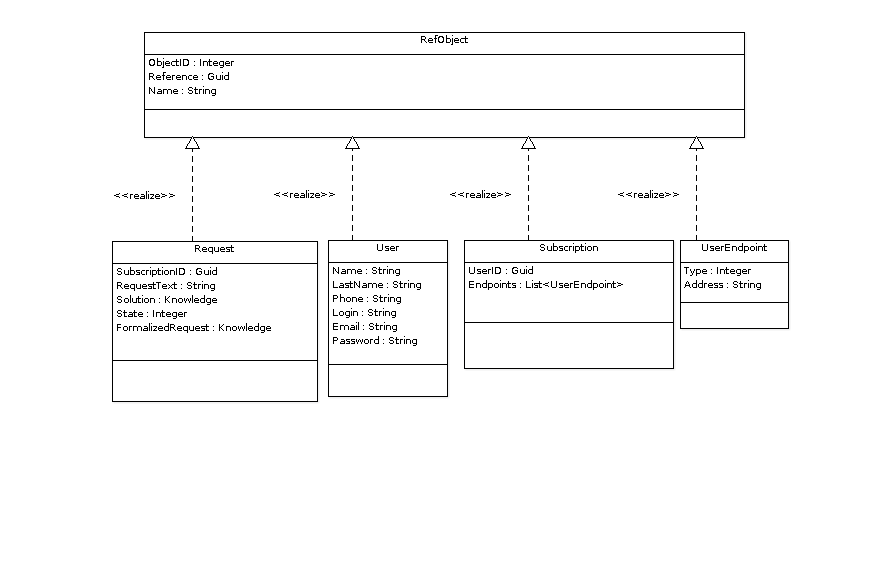
\includegraphics [scale=0.8,angle=90, origin=c] {interface-model}
  \caption{Диаграмма классов интерфейсной модели} 
  \label{img:interface-model}  
\end{figure}

Рассмотрим несколько объектов, например, Request (Запрос). Он предназначен для хранения запроса пользователя:
\begin{itemize}
	\item SubscriptionID~--- идентификатор подписки, ссылка на сущность Subscription (подписка);
	\item RequestText~--- запрос пользователя в виде текста;
	\item Solution~--- описание решения запроса пользователя;
	\item State~--- статус запроса (например, «поиск решения»);
	\item FormalizedRequest~--- ссылка на формализованный запрос.
\end{itemize} \par
Subscription (подписка) содержит информацию о подписке пользователя на информирование о событиях. Список точек оповещения (Endpoints), благодаря которым система будет предоставлять информацию пользователю о состоянии его запроса. Точка оповещения описывается набором параметров из Type (тип)~--- тип точки связи с пользователем (например, веб-сервис) и Address (адрес)~--- адрес точки связи с пользователем.

%=======================
%======APPENDIX B=======
%=======================
\chapter{Описание модуля Goal (Цель) и Action (Действия)} \label{AppendixB}
Action (Действие) является базовым классом для WayToThink или Critic. Он описывает общие методы этих классов: start (запуск); stop (остановка) и apply (применение)~--- метод, который производит работу над контекстом и изменяет данные. На рисунку \ref{img:ActionClass} представлена диаграмма классов Action, где отображена связь с Critic и WayToThink.
\begin{figure} [h] 
  \center
  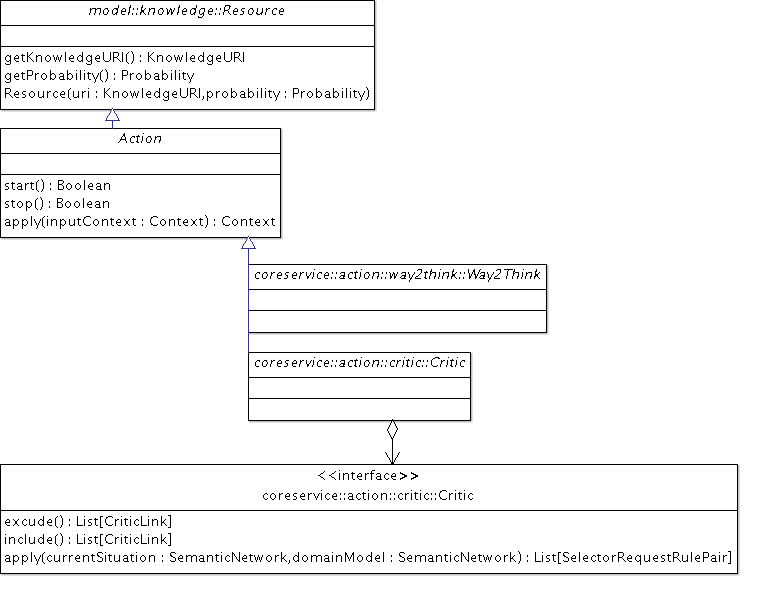
\includegraphics [scale=0.65] {ActionClass}
  \caption{Диаграмма классов Action} 
  \label{img:ActionClass}  
\end{figure}

Goal (Цель) является набором вероятностных предикатов и последовательностью How-To необходимых для того, чтобы достичь цель. Goal и How-To тесно связаны. На рисунке \ref{img:goal} показан состав Goal. Goal состоит из:
\begin{enumerate}
	\item Parameters~--- параметры, которые используются предикатами для выполнения;
	\item Precondition~--- условия, которые должны быть выполнены до начала основной проверки (Exit criteria);
	\item Entry criteria~--- входной критерий, предикат, который определяет, что цель активировалась;
	\item Exit criteria~--- условия, когда цель считается выполненной;
	\item PostCondition~--- дополнительные условия для выхода;
	\item HowTo~--- набор решения. Список путей решения.
\end{enumerate}

\begin{figure} [h] 
  \center
  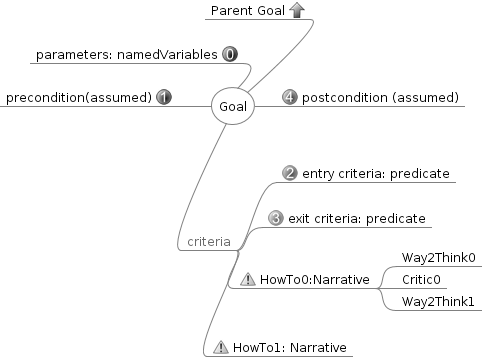
\includegraphics [scale=1.0, origin=c] {goal}
  \caption{Диаграмма классов Goal} 
  \label{img:goal}  
\end{figure} \par
\clearpage
\textbf{Типы предикатов}. В решении используется 3 типа логических предикатов: and (и), or (или), not (отрицание). Представление Goal в SemanticNetwork показано на диаграмме \ref{img:2_0_GoalHowToConcept}.

\begin{figure} [h] 
  \center
  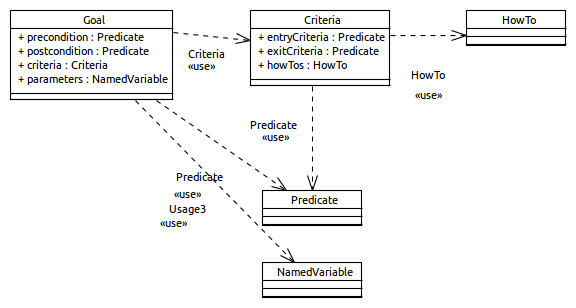
\includegraphics [scale=1.0, origin=c] {2_0_GoalHowToConcept}
  \caption{Диаграмма места Goal в SemanticNetwork (Семантической сети)} 
  \label{img:2_0_GoalHowToConcept}  
\end{figure}

Основная цель системы~--- помочь пользователю. Все остальные цели являются подцелями основной: разрешить инцидент, понять тип инцидента, найти решение инцидента \etc.

%=======================
%======APPENDIX D=======
%=======================
\chapter{Рецепты решений} \label{AppendixDHowTo}
Рецепты решений представляют собой последовательность действий выполняемых для разрешения проблемы, описанной в инциденте. 
Было разработано два типа HowTo (рецепт решения): ValueHowTo~--- содержит в себе простое значение; FunctionalHowTo~--- содержит в себе функцию. \par
FunctionalHowTo состоит из следующих частей:
\begin{enumerate}
	\item FunctionalBody~--- тело функции, описывающий содержание функции;
	\item InputParameters~--- входные параметры функции;
	\item OutputParameters~--- выходные параметры.
\end{enumerate} \par
Комбинация FunctionaHowTo и ValueHowTo является рецептом решения. Например, решение проблемы неработающего сегмента кластера в формате для специалиста технической поддержки.
\begin{itemize}
	\item Войти на сервер U1;
	\item Запустить утилиту 12 для Windows Servers;
	\item Открыть вкладку 1;
	\item Перейти на All Managed Server, найти нужный Server из правой панели, открыть свойства сервера;
	\item Нажать на Backup Exec Services;
	\item Выберите проблемный сегмент кластера;
	\item Нажмите Restart all Services;
	\item Подождите и проверьте статус.
\end{itemize} \par
Преобразованный в формат HowTo данный рецепт решения будет выглядеть как показано ниже.

\begin{lstlisting}
	login:howto{
  Parameters:[

    {Key:'ScriptName',
    Value:'LogonScript.bat'},
    {Key:'Description',
    Value:'Logon to server'}
  ]

  InputParameters:[
    {Key:'ServerName',
    Value:'U1'},
    {Key:'UserName',
    Value:'MyUser'}
  ]

  OutputParameters:[
    {Key:'SessionID',
    Value:'SSSE12'},

  ]
}

launch:howto{
  Parameters:[

    {Key:'ScriptName',
    Value:'LaunchScript.bat'},
    {Key:'Description',
    Value:'Launch the application'}
  ]

  InputParameters:[
    {Key:'ExecName',
    Value:'Utility12.exe'},
  ]

  OutputParameters:[
    {Key:'SessionID',
    Value:'SSSE12'},

  ]
}
\end{lstlisting}
%=======================
%======APPENDIX E=======
%=======================
\clearpage
\chapter{Экспериментальные данные}\label{AppendixE}
Здесь приведена лишь часть экспериментальных данных (Общая длина файла примерно 10000 инцидентов). 
\begin{longtable}{|p{5cm}|p{6cm}|p{5cm}|}
 \caption[Описание экспериментальных данных]{Описание экспериментальных данных}\label{ExpData} \\ 
 \hline
 
 \multicolumn{1}{|c|}{\textbf{Класс проблемы}}& \multicolumn{1}{c|}{\textbf{
 Описание проблемы}} & \multicolumn{1}{c|}{\textbf{
 \% успешных}}  \\ \hline 
\endfirsthead
\multicolumn{2}{c}%
{{\bfseries \tablename\ \thetable{} -- продолжение}} \\
\hline \multicolumn{1}{|c|}{\textbf{Входное предложение}} &
\multicolumn{1}{c|}{\textbf{Описание}}  \\ \hline 
\endhead

\endfoot

\hline \hline
\endlastfoot
\hline

Проблема с ПО   &  & 64\% \\
 \hline Проблемы во время работы &  &  10\% \\
  \hline Как сделать&  & 10\% \\
    \hline         &    Hi NAS Admin,Please connect following groups to the shared disk listed below and configure security permissions.    &  Разрешена, уточнены, выявлены концепции: connect, following groups, shared disks.  \\
     \hline         &    Failed LOT OrderReciever.   &  Не решено, не достаточно информации.  \\
      \hline         &    Delivery of request VCC395244Service: Network Services - LAN - LAN Order of AliasService manager.   &   Не разрешено, не выявлено ключевых концепций проблемы, например, failed, error.  \\
       \hline         &    User needs latest version of Catia v5 Teamcenter.reinstalled installed.He has been instructed by the design support to ask for an installation.   &  Разрешена, выявлены концепции: user, needs, Catia v5.  \\
        \hline         &    User should have gotten WordFinder(9, En-Sv/ v-En Affärsekonomisk) and WordFinder(9, Ne-Sv Sv-Ne, Nederländska) installed but that is not the case. please install the applciation for the userName: DELVA.   &  Не разрешено, непонятно, что делать с первым пользователем.  \\
         \hline         &    What do you want to do?: Add new aliasHost name on host that alias is wanted to.   &  Разрешена, выявлены концепции: add, aliashost.  \\
   \hline
   \hline     ...    &   ...   & ... \\
Проблема с оборудованием &  & 0\% \\
 \hline         &    VCC ParamServicesFailingService         The status of the lcfd service is Degraded.     Critical.   &  Не разрешено, проблема с аппаратной частью.  \\
\hline         &    HeartBeat EndpointUnreachable   Tivoli lcf endpoint is unreachable.   &  Не разрешено, проблема с аппаратной частью.  \\
\hline         &    TMW ProcessorBusy.   &  Не разрешено, не достаточное описание проблемы.  \\
\hline     ...    &   ...   & ... \\
 \hline
Установить новое ПО    &    & 100\% \\
\hline         &    HyperionFM SmartView 9.3.3I need a new version of a software. HyperionFM SmartView 9.3.3 is the new version I need..   &  Разрешено, выявлены концепции: i, need, SmartView 9.3.3.  \\

\hline         &    User requsts internet explorer 8 to be installed.   &  Разрешено, выявлены концепции: user, requests, internet explorer 8.  \\
\hline         &    The installation of Winrar that I got this afternoon did go wrong. During installation nothing else was running. When I tried to start Winrar I got the fault message that is attached here.   &  Разрешено, выявлены концепции: winrar, installation, did wrong. Решение~--- переустановить. \\

\hline         &    User got wrong homepage. He want to have vcc-intranet as homepage, but got something other "email-related".   &  Разрешено, выявлены концепции: user, got wrong, homepage, he, want, vcc-intranet.  

\\

\hline         &    Users IE8 has dissapred, please reinstall the application for him.   &  Разрешено, выявлены концепции: IE8, dissapered, please, reinstall, for him.  

\\

\hline         &    User has not got IE8 installed yet.   &  Разрешено, выявлены концепции: IE8, user, has not got, for him.  

\\

\hline         &    User need launged pack for east asianplease see attached picture.   &  Разрешено, выявлены концепции: user, need, language pack, east asian.  
\\



\hline     ...    &   ...   & ... \\



 \hline Проблема с печатью    &     & 80\% \\
 
 \hline         &    User is not able to print from TIE. He is using compability view in IE8Name.   &  Разрешено, выявлены концепции: user, not able, print, TIE, compability, IE8.  \\
 
  \hline         &    User is not able to print with PDF995. he gets a error saying Could not load.   &  Разрешено, выявлены концепции: user, not able, print, PDF995.  \\
 
 \hline         &    According to IM3548717 user couldt print from SAP, now she can print from SAP, but other programs such as Outlook and excel wont work, getting errormessage "unable to connect.   &  Разрешено, выявлены концепции: user, getting, error message, unable, connect.  \\
 
 \hline         &    User is trying to print to PR40378 from Adobe Reader and Powerpoint but gets "printing failed - no pages selected".   &  Не разрешено, выявлены концепции: user, trying, print, Adobe Reader, PowerPoint, printing, failed. Неоднозначность запроса для системы.  \\

 
\hline     ...    &   ...   & ... \\
  \hline Нет доступа         &       & 100\% \\
  
   \hline         &    User gets Invalid Login when trying to logon to Teamcenter. He has got a new password and changed it on the new CDSID page but it still does not work.    &  Разрешено, создан новый логин. \\

   \hline         &   Problems with 3G modems after migration: "Mobile connection not possible. Ensure that no other programs are using your selected device, and try again in a short while" The user is a agent working at the UK.    & Разрешено, система уточнила проблему в диалоге с пользователем. \\

   \hline         &    User had received wrong application. User has ordered Wordfinder Business Economical. However she received wrong version, she received Wordfinder Tehcnical instead of Business Economical.   &  Разрешена, уточнены, выявлены концепции: Wordfinder Tehcnical,  Business Economical  \\
  \hline         &    User needs to have pdf 995 re-installed please.    & Разрешено. Выявлены концепции pdf, need и install. \\
  \hline         &    User dosn't have the Intel proset wireless application installed on his computer.    & Разрешено, выявлены концепции: doesn't have,  Intel proset. \\
  \hline         &    "Teamcenter \& tc vis" have been uninstalled somehow from users clientPlease reinstall.    &  Разрешено, выявлены концепции: reinstall, users, "Teamcenter \& tc vis"\\
  \hline         &    User can no longer access any wireless networksproblem with user profile, needs to be reconfigured, installed.    & Разрешено. Найдены концепции:  wireless networksproblem, user, user profile, reconfigured.\\
\hline     ...    &   ...   & ... \\

 
  \hline
  \end{longtable}
  

%=======================
%======APPENDIX F=======
%=======================
\clearpage
\chapter{Свидетельство о регистрации}\label{AppendixF}


\begin{figure} [h] 
  \center
  
\includegraphics [scale=0.12] {RegistrationStatement}
  \caption{Свидетельство о регистрации} 
  \label{img:RegistrationStatement}  
\end{figure}



%=======================
%======APPENDIX G=======
%=======================
\clearpage
\chapter{Акт о внедрении}\label{AppendixG}


\begin{figure} [h] 
  \center
  
\includegraphics [scale=0.12] {ActVnedr}
  \caption{Акт о внедрении} 
  \label{img:ActVnedr}  
\end{figure}

